\documentclass[oneside]{amsart}
\usepackage{amsmath, amsfonts, amsthm, amssymb}
\usepackage{color}
\usepackage{tikz}
\usetikzlibrary{arrows,decorations.pathmorphing,backgrounds,positioning,fit,petri}
\usepackage[pdftex,colorlinks,citecolor=blue]{hyperref}

\begin{document}

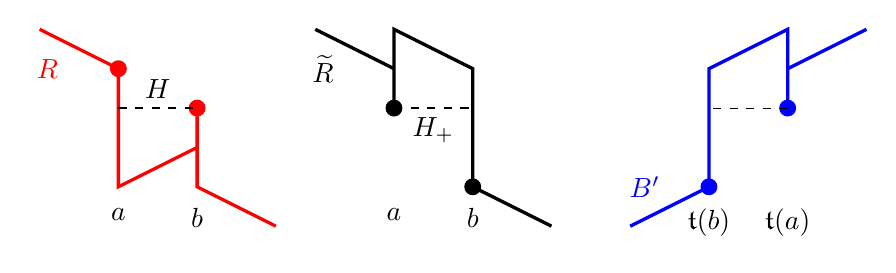
\begin{tikzpicture}%
%
\begin{scope}
\coordinate (A) at (0,3); % (1,2)--(2.5,2) (2.9,1)--(4.1,1)
\coordinate (B) at (1,2.5);
\coordinate (B1) at (1,2.5);
\coordinate (B2) at (1,2);
\coordinate (B3) at (1,1);
\coordinate (C) at (2.9,1);
\coordinate (C2) at (2,2);
\coordinate (Z2) at (1.5,2);
\coordinate (C3) at (2,1.5);
\coordinate (C4) at (2,1);
\coordinate (D) at (3,.5);
\coordinate (X) at (1,.85);
\coordinate (Y) at (2,.85);
\coordinate (Z) at (.1,2.5);
\draw[very thick,red] (A)--(B1)--(B3)--(C3)--(C2)--(C4)--(D);
\draw[red,fill] (B1) circle[radius=1mm];
\draw[red,fill] (C2) circle[radius=1mm];
\draw (X) node[below]{$a$};
\draw (Y) node[below]{$b$};
\draw (Z2) node[above]{$H$};
\draw[thick,dashed] (B2)--(C2);
\draw[red] (Z) node{$R$};
\end{scope}
%
\begin{scope}[xshift=3.5cm]
\coordinate (A) at (0,3); % (1,2)--(2.5,2) (2.9,1)--(4.1,1)
\coordinate (B) at (1,2.5);
\coordinate (B1) at (1,2.5);
\coordinate (B0) at (1,3);
\coordinate (B2) at (1,2);
\coordinate (B3) at (1,1);
\coordinate (C) at (2.9,1);
\coordinate (C1) at (2,2.5);
\coordinate (C2) at (2,2);
\coordinate (C3) at (2,1.5);
\coordinate (C4) at (2,1);
\coordinate (D) at (3,.5);
\coordinate (Z) at (.1,2.5);
\coordinate (Z2) at (1.5,2);
\coordinate (X) at (1,.85);
\coordinate (Y) at (2,.85);
\draw (X) node[below]{$a$};
\draw (Y) node[below]{$b$};
\draw (Z2) node[below]{$H_+$};
\draw[fill] (B2) circle[radius=1mm];
\draw[fill] (C4) circle[radius=1mm];
\draw[thick,dashed] (B2)--(C2);
\draw[very thick] (A)--(B1)--(B2)--(B0)--(C1)--(C4)--(D);
\draw (Z) node{$\widetilde R$};
\end{scope}
%
%
\begin{scope}[xshift=10.5cm,xscale=-1]
\coordinate (A) at (0,3); % (1,2)--(2.5,2) (2.9,1)--(4.1,1)
\coordinate (B) at (1,2.5);
\coordinate (B1) at (1,2.5);
\coordinate (B0) at (1,3);
\coordinate (B2) at (1,2);
\coordinate (B3) at (1,1);
\coordinate (C) at (2.9,1);
\coordinate (C1) at (2,2.5);
\coordinate (C2) at (2,2);
\coordinate (C3) at (2,1.5);
\coordinate (C4) at (2,1);
\coordinate (D) at (3,.5);
\coordinate (Z) at (2.5,1);
\coordinate (X) at (1,.85);
\coordinate (Y) at (2,.85);
\draw (X) node[below]{$\mathfrak t(a)$};
\draw (Y) node[below]{$\mathfrak t(b)$};
\draw[fill,blue] (B2) circle[radius=1mm];
\draw[fill,blue] (C4) circle[radius=1mm];
\draw[dashed,black] (B2)--(C2);
\draw[very thick,blue] (A)--(B1)--(B2)--(B0)--(C1)--(C4)--(D);
\draw[blue] (Z) node[left]{$B'$};
\end{scope}
%
\end{tikzpicture}

\end{document}